\documentclass[11pt,compress,t,notes=noshow, xcolor=table]{beamer}
\documentclass[11pt,compress,t,notes=noshow, xcolor=table]{beamer}
\usepackage[]{graphicx}\usepackage[]{color}
% maxwidth is the original width if it is less than linewidth
% otherwise use linewidth (to make sure the graphics do not exceed the margin)
\makeatletter
\def\maxwidth{ %
  \ifdim\Gin@nat@width>\linewidth
    \linewidth
  \else
    \Gin@nat@width
  \fi
}
\makeatother

\definecolor{fgcolor}{rgb}{0.345, 0.345, 0.345}
\newcommand{\hlnum}[1]{\textcolor[rgb]{0.686,0.059,0.569}{#1}}%
\newcommand{\hlstr}[1]{\textcolor[rgb]{0.192,0.494,0.8}{#1}}%
\newcommand{\hlcom}[1]{\textcolor[rgb]{0.678,0.584,0.686}{\textit{#1}}}%
\newcommand{\hlopt}[1]{\textcolor[rgb]{0,0,0}{#1}}%
\newcommand{\hlstd}[1]{\textcolor[rgb]{0.345,0.345,0.345}{#1}}%
\newcommand{\hlkwa}[1]{\textcolor[rgb]{0.161,0.373,0.58}{\textbf{#1}}}%
\newcommand{\hlkwb}[1]{\textcolor[rgb]{0.69,0.353,0.396}{#1}}%
\newcommand{\hlkwc}[1]{\textcolor[rgb]{0.333,0.667,0.333}{#1}}%
\newcommand{\hlkwd}[1]{\textcolor[rgb]{0.737,0.353,0.396}{\textbf{#1}}}%
\let\hlipl\hlkwb

\usepackage{framed}
\makeatletter
\newenvironment{kframe}{%
 \def\at@end@of@kframe{}%
 \ifinner\ifhmode%
  \def\at@end@of@kframe{\end{minipage}}%
  \begin{minipage}{\columnwidth}%
 \fi\fi%
 \def\FrameCommand##1{\hskip\@totalleftmargin \hskip-\fboxsep
 \colorbox{shadecolor}{##1}\hskip-\fboxsep
     % There is no \\@totalrightmargin, so:
     \hskip-\linewidth \hskip-\@totalleftmargin \hskip\columnwidth}%
 \MakeFramed {\advance\hsize-\width
   \@totalleftmargin\z@ \linewidth\hsize
   \@setminipage}}%
 {\par\unskip\endMakeFramed%
 \at@end@of@kframe}
\makeatother

\definecolor{shadecolor}{rgb}{.97, .97, .97}
\definecolor{messagecolor}{rgb}{0, 0, 0}
\definecolor{warningcolor}{rgb}{1, 0, 1}
\definecolor{errorcolor}{rgb}{1, 0, 0}
\newenvironment{knitrout}{}{} % an empty environment to be redefined in TeX

\usepackage{alltt}
\newcommand{\SweaveOpts}[1]{}  % do not interfere with LaTeX
\newcommand{\SweaveInput}[1]{} % because they are not real TeX commands
\newcommand{\Sexpr}[1]{}       % will only be parsed by R
\newcommand{\xmark}{\ding{55}}%


\usepackage[english]{babel}
\usepackage[utf8]{inputenc}

\usepackage{dsfont}
\usepackage{verbatim}
\usepackage{amsmath}
\usepackage{amsfonts}
\usepackage{amssymb}
\usepackage{bm}
\usepackage{csquotes}
\usepackage{multirow}
\usepackage{longtable}
\usepackage{booktabs}
\usepackage{enumerate}
\usepackage[absolute,overlay]{textpos}
\usepackage{psfrag}
\usepackage{algorithm}
\usepackage{algpseudocode}
\usepackage{eqnarray}
\usepackage{arydshln}
\usepackage{tabularx}
\usepackage{placeins}
\usepackage{tikz}
\usepackage{setspace}
\usepackage{colortbl}
\usepackage{mathtools}
\usepackage{wrapfig}
\usepackage{bm}
\usepackage{amsmath}
\usepackage{pifont}

\usetikzlibrary{shapes,arrows,automata,positioning,calc,chains,trees, shadows}
\tikzset{
  %Define standard arrow tip
  >=stealth',
  %Define style for boxes
  punkt/.style={
    rectangle,
    rounded corners,
    draw=black, very thick,
    text width=6.5em,
    minimum height=2em,
    text centered},
  % Define arrow style
  pil/.style={
    ->,
    thick,
    shorten <=2pt,
    shorten >=2pt,}
}

\usepackage{subfig}

% Defines macros and environments
\usepackage{../../style/lmu-lecture}


\let\code=\texttt
\let\proglang=\textsf

\setkeys{Gin}{width=0.9\textwidth}

\setbeamertemplate{frametitle}{\expandafter\uppercase\expandafter\insertframetitle}

% This file is included in slides and exercises

% Rarely used fontstyle for R packages, used only in 
% - forests/slides-forests-benchmark.tex
% - exercises/single-exercises/methods_l_1.Rnw
% - slides/cart/attic/slides_extra_trees.Rnw
\newcommand{\pkg}[1]{{\fontseries{b}\selectfont #1}}

% Spacing helpers, used often (mostly in exercises for \dlz)
\newcommand{\lz}{\vspace{0.5cm}} % vertical space (used often in slides)
\newcommand{\dlz}{\vspace{1cm}}  % double vertical space (used often in exercises, never in slides)
\newcommand{\oneliner}[1] % Oneliner for important statements, used e.g. in iml, algods
{\begin{block}{}\begin{center}\begin{Large}#1\end{Large}\end{center}\end{block}}

% Don't know if this is used or needed, remove?
% textcolor that works in mathmode
% https://tex.stackexchange.com/a/261480
% Used e.g. in forests/slides-forests-bagging.tex
% [...] \textcolor{blue}{\tfrac{1}{M}\sum^M_{m} [...]
% \makeatletter
% \renewcommand*{\@textcolor}[3]{%
%   \protect\leavevmode
%   \begingroup
%     \color#1{#2}#3%
%   \endgroup
% }
% \makeatother






% latex-math includes as needed
% dependencies: amsmath, amssymb, dsfont
% math spaces
\ifdefined\N
\renewcommand{\N}{\mathds{N}} % N, naturals
\else \newcommand{\N}{\mathds{N}} \fi
\newcommand{\Z}{\mathds{Z}} % Z, integers
\newcommand{\Q}{\mathds{Q}} % Q, rationals
\newcommand{\R}{\mathds{R}} % R, reals
\ifdefined\C
\renewcommand{\C}{\mathds{C}} % C, complex
\else \newcommand{\C}{\mathds{C}} \fi
\newcommand{\continuous}{\mathcal{C}} % C, space of continuous functions
\newcommand{\M}{\mathcal{M}} % machine numbers
\newcommand{\epsm}{\epsilon_m} % maximum error

% counting / finite sets
\newcommand{\setzo}{\{0, 1\}} % set 0, 1
\newcommand{\setmp}{\{-1, +1\}} % set -1, 1
\newcommand{\unitint}{[0, 1]} % unit interval

% basic math stuff
\newcommand{\xt}{\tilde x} % x tilde
\newcommand{\argmin}{\mathop{\mathrm{arg\,min}}} % argmin
\newcommand{\argmax}{\mathop{\mathrm{arg\,max}}} % argmax
\newcommand{\argminlim}{\argmin\limits} % argmin with limits
\newcommand{\argmaxlim}{\argmax\limits} % argmax with limits
\newcommand{\sign}{\operatorname{sign}} % sign, signum
\newcommand{\I}{\mathbb{I}} % I, indicator
\newcommand{\order}{\mathcal{O}} % O, order
\newcommand{\bigO}{\mathcal{O}} % Big-O Landau
\newcommand{\littleo}{{o}} % Little-o Landau
\newcommand{\pd}[2]{\frac{\partial{#1}}{\partial #2}} % partial derivative
\newcommand{\floorlr}[1]{\left\lfloor #1 \right\rfloor} % floor
\newcommand{\ceillr}[1]{\left\lceil #1 \right\rceil} % ceiling
\newcommand{\indep}{\perp \!\!\! \perp} % independence symbol

% sums and products
\newcommand{\sumin}{\sum\limits_{i=1}^n} % summation from i=1 to n
\newcommand{\sumim}{\sum\limits_{i=1}^m} % summation from i=1 to m
\newcommand{\sumjn}{\sum\limits_{j=1}^n} % summation from j=1 to p
\newcommand{\sumjp}{\sum\limits_{j=1}^p} % summation from j=1 to p
\newcommand{\sumik}{\sum\limits_{i=1}^k} % summation from i=1 to k
\newcommand{\sumkg}{\sum\limits_{k=1}^g} % summation from k=1 to g
\newcommand{\sumjg}{\sum\limits_{j=1}^g} % summation from j=1 to g
\newcommand{\summM}{\sum\limits_{m=1}^M} % summation from m=1 to M
\newcommand{\meanin}{\frac{1}{n} \sum\limits_{i=1}^n} % mean from i=1 to n
\newcommand{\meanim}{\frac{1}{m} \sum\limits_{i=1}^m} % mean from i=1 to n
\newcommand{\meankg}{\frac{1}{g} \sum\limits_{k=1}^g} % mean from k=1 to g
\newcommand{\meanmM}{\frac{1}{M} \sum\limits_{m=1}^M} % mean from m=1 to M
\newcommand{\prodin}{\prod\limits_{i=1}^n} % product from i=1 to n
\newcommand{\prodkg}{\prod\limits_{k=1}^g} % product from k=1 to g
\newcommand{\prodjp}{\prod\limits_{j=1}^p} % product from j=1 to p

% linear algebra
\newcommand{\one}{\bm{1}} % 1, unitvector
\newcommand{\zero}{\mathbf{0}} % 0-vector
\newcommand{\id}{\bm{I}} % I, identity
\newcommand{\diag}{\operatorname{diag}} % diag, diagonal
\newcommand{\trace}{\operatorname{tr}} % tr, trace
\newcommand{\spn}{\operatorname{span}} % span
\newcommand{\scp}[2]{\left\langle #1, #2 \right\rangle} % <.,.>, scalarproduct
\newcommand{\mat}[1]{\begin{pmatrix} #1 \end{pmatrix}} % short pmatrix command
\newcommand{\Amat}{\mathbf{A}} % matrix A
\newcommand{\Deltab}{\mathbf{\Delta}} % error term for vectors

% basic probability + stats
\renewcommand{\P}{\mathds{P}} % P, probability
\newcommand{\E}{\mathds{E}} % E, expectation
\newcommand{\var}{\mathsf{Var}} % Var, variance
\newcommand{\cov}{\mathsf{Cov}} % Cov, covariance
\newcommand{\corr}{\mathsf{Corr}} % Corr, correlation
\newcommand{\normal}{\mathcal{N}} % N of the normal distribution
\newcommand{\iid}{\overset{i.i.d}{\sim}} % dist with i.i.d superscript
\newcommand{\distas}[1]{\overset{#1}{\sim}} % ... is distributed as ...

% machine learning
\newcommand{\Xspace}{\mathcal{X}} % X, input space
\newcommand{\Yspace}{\mathcal{Y}} % Y, output space
\newcommand{\Zspace}{\mathcal{Z}} % Z, space of sampled datapoints
\newcommand{\nset}{\{1, \ldots, n\}} % set from 1 to n
\newcommand{\pset}{\{1, \ldots, p\}} % set from 1 to p
\newcommand{\gset}{\{1, \ldots, g\}} % set from 1 to g
\newcommand{\Pxy}{\mathbb{P}_{xy}} % P_xy
\newcommand{\Exy}{\mathbb{E}_{xy}} % E_xy: Expectation over random variables xy
\newcommand{\xv}{\mathbf{x}} % vector x (bold)
\newcommand{\xtil}{\tilde{\mathbf{x}}} % vector x-tilde (bold)
\newcommand{\yv}{\mathbf{y}} % vector y (bold)
\newcommand{\xy}{(\xv, y)} % observation (x, y)
\newcommand{\xvec}{\left(x_1, \ldots, x_p\right)^\top} % (x1, ..., xp)
\newcommand{\Xmat}{\mathbf{X}} % Design matrix
\newcommand{\allDatasets}{\mathds{D}} % The set of all datasets
\newcommand{\allDatasetsn}{\mathds{D}_n}  % The set of all datasets of size n
\newcommand{\D}{\mathcal{D}} % D, data
\newcommand{\Dn}{\D_n} % D_n, data of size n
\newcommand{\Dtrain}{\mathcal{D}_{\text{train}}} % D_train, training set
\newcommand{\Dtest}{\mathcal{D}_{\text{test}}} % D_test, test set
\newcommand{\xyi}[1][i]{\left(\xv^{(#1)}, y^{(#1)}\right)} % (x^i, y^i), i-th observation
\newcommand{\Dset}{\left( \xyi[1], \ldots, \xyi[n]\right)} % {(x1,y1)), ..., (xn,yn)}, data
\newcommand{\defAllDatasetsn}{(\Xspace \times \Yspace)^n} % Def. of the set of all datasets of size n
\newcommand{\defAllDatasets}{\bigcup_{n \in \N}(\Xspace \times \Yspace)^n} % Def. of the set of all datasets
\newcommand{\xdat}{\left\{ \xv^{(1)}, \ldots, \xv^{(n)}\right\}} % {x1, ..., xn}, input data
\newcommand{\ydat}{\left\{ \yv^{(1)}, \ldots, \yv^{(n)}\right\}} % {y1, ..., yn}, input data
\newcommand{\yvec}{\left(y^{(1)}, \hdots, y^{(n)}\right)^\top} % (y1, ..., yn), vector of outcomes
\newcommand{\greekxi}{\xi} % Greek letter xi
\renewcommand{\xi}[1][i]{\xv^{(#1)}} % x^i, i-th observed value of x
\newcommand{\yi}[1][i]{y^{(#1)}} % y^i, i-th observed value of y
\newcommand{\xivec}{\left(x^{(i)}_1, \ldots, x^{(i)}_p\right)^\top} % (x1^i, ..., xp^i), i-th observation vector
\newcommand{\xj}{\xv_j} % x_j, j-th feature
\newcommand{\xjvec}{\left(x^{(1)}_j, \ldots, x^{(n)}_j\right)^\top} % (x^1_j, ..., x^n_j), j-th feature vector
\newcommand{\phiv}{\mathbf{\phi}} % Basis transformation function phi
\newcommand{\phixi}{\mathbf{\phi}^{(i)}} % Basis transformation of xi: phi^i := phi(xi)

%%%%%% ml - models general
\newcommand{\lamv}{\bm{\lambda}} % lambda vector, hyperconfiguration vector
\newcommand{\Lam}{\bm{\Lambda}}	 % Lambda, space of all hpos
% Inducer / Inducing algorithm
\newcommand{\preimageInducer}{\left(\defAllDatasets\right)\times\Lam} % Set of all datasets times the hyperparameter space
\newcommand{\preimageInducerShort}{\allDatasets\times\Lam} % Set of all datasets times the hyperparameter space
% Inducer / Inducing algorithm
\newcommand{\ind}{\mathcal{I}} % Inducer, inducing algorithm, learning algorithm

% continuous prediction function f
\newcommand{\ftrue}{f_{\text{true}}}  % True underlying function (if a statistical model is assumed)
\newcommand{\ftruex}{\ftrue(\xv)} % True underlying function (if a statistical model is assumed)
\newcommand{\fx}{f(\xv)} % f(x), continuous prediction function
\newcommand{\fdomains}{f: \Xspace \rightarrow \R^g} % f with domain and co-domain
\newcommand{\Hspace}{\mathcal{H}} % hypothesis space where f is from
\newcommand{\fbayes}{f^{\ast}} % Bayes-optimal model
\newcommand{\fxbayes}{f^{\ast}(\xv)} % Bayes-optimal model
\newcommand{\fkx}[1][k]{f_{#1}(\xv)} % f_j(x), discriminant component function
\newcommand{\fh}{\hat{f}} % f hat, estimated prediction function
\newcommand{\fxh}{\fh(\xv)} % fhat(x)
\newcommand{\fxt}{f(\xv ~|~ \thetav)} % f(x | theta)
\newcommand{\fxi}{f\left(\xv^{(i)}\right)} % f(x^(i))
\newcommand{\fxih}{\hat{f}\left(\xv^{(i)}\right)} % f(x^(i))
\newcommand{\fxit}{f\left(\xv^{(i)} ~|~ \thetav\right)} % f(x^(i) | theta)
\newcommand{\fhD}{\fh_{\D}} % fhat_D, estimate of f based on D
\newcommand{\fhDtrain}{\fh_{\Dtrain}} % fhat_Dtrain, estimate of f based on D
\newcommand{\fhDnlam}{\fh_{\Dn, \lamv}} %model learned on Dn with hp lambda
\newcommand{\fhDlam}{\fh_{\D, \lamv}} %model learned on D with hp lambda
\newcommand{\fhDnlams}{\fh_{\Dn, \lamv^\ast}} %model learned on Dn with optimal hp lambda
\newcommand{\fhDlams}{\fh_{\D, \lamv^\ast}} %model learned on D with optimal hp lambda

% discrete prediction function h
\newcommand{\hx}{h(\xv)} % h(x), discrete prediction function
\newcommand{\hh}{\hat{h}} % h hat
\newcommand{\hxh}{\hat{h}(\xv)} % hhat(x)
\newcommand{\hxt}{h(\xv | \thetav)} % h(x | theta)
\newcommand{\hxi}{h\left(\xi\right)} % h(x^(i))
\newcommand{\hxit}{h\left(\xi ~|~ \thetav\right)} % h(x^(i) | theta)
\newcommand{\hbayes}{h^{\ast}} % Bayes-optimal classification model
\newcommand{\hxbayes}{h^{\ast}(\xv)} % Bayes-optimal classification model

% yhat
\newcommand{\yh}{\hat{y}} % yhat for prediction of target
\newcommand{\yih}{\hat{y}^{(i)}} % yhat^(i) for prediction of ith targiet
\newcommand{\resi}{\yi- \yih}

% theta
\newcommand{\thetah}{\hat{\theta}} % theta hat
\newcommand{\thetav}{\bm{\theta}} % theta vector
\newcommand{\thetavh}{\bm{\hat\theta}} % theta vector hat
\newcommand{\thetat}[1][t]{\thetav^{[#1]}} % theta^[t] in optimization
\newcommand{\thetatn}[1][t]{\thetav^{[#1 +1]}} % theta^[t+1] in optimization
\newcommand{\thetahDnlam}{\thetavh_{\Dn, \lamv}} %theta learned on Dn with hp lambda
\newcommand{\thetahDlam}{\thetavh_{\D, \lamv}} %theta learned on D with hp lambda
\newcommand{\mint}{\min_{\thetav \in \Theta}} % min problem theta
\newcommand{\argmint}{\argmin_{\thetav \in \Theta}} % argmin theta

% densities + probabilities
% pdf of x
\newcommand{\pdf}{p} % p
\newcommand{\pdfx}{p(\xv)} % p(x)
\newcommand{\pixt}{\pi(\xv~|~ \thetav)} % pi(x|theta), pdf of x given theta
\newcommand{\pixit}[1][i]{\pi\left(\xi[#1] ~|~ \thetav\right)} % pi(x^i|theta), pdf of x given theta
\newcommand{\pixii}[1][i]{\pi\left(\xi[#1]\right)} % pi(x^i), pdf of i-th x

% pdf of (x, y)
\newcommand{\pdfxy}{p(\xv,y)} % p(x, y)
\newcommand{\pdfxyt}{p(\xv, y ~|~ \thetav)} % p(x, y | theta)
\newcommand{\pdfxyit}{p\left(\xi, \yi ~|~ \thetav\right)} % p(x^(i), y^(i) | theta)

% pdf of x given y
\newcommand{\pdfxyk}[1][k]{p(\xv | y= #1)} % p(x | y = k)
\newcommand{\lpdfxyk}[1][k]{\log p(\xv | y= #1)} % log p(x | y = k)
\newcommand{\pdfxiyk}[1][k]{p\left(\xi | y= #1 \right)} % p(x^i | y = k)

% prior probabilities
\newcommand{\pik}[1][k]{\pi_{#1}} % pi_k, prior
\newcommand{\lpik}[1][k]{\log \pi_{#1}} % log pi_k, log of the prior
\newcommand{\pit}{\pi(\thetav)} % Prior probability of parameter theta

% posterior probabilities
\newcommand{\post}{\P(y = 1 ~|~ \xv)} % P(y = 1 | x), post. prob for y=1
\newcommand{\postk}[1][k]{\P(y = #1 ~|~ \xv)} % P(y = k | y), post. prob for y=k
\newcommand{\pidomains}{\pi: \Xspace \rightarrow \unitint} % pi with domain and co-domain
\newcommand{\pibayes}{\pi^{\ast}} % Bayes-optimal classification model
\newcommand{\pixbayes}{\pi^{\ast}(\xv)} % Bayes-optimal classification model
\newcommand{\pix}{\pi(\xv)} % pi(x), P(y = 1 | x)
\newcommand{\piv}{\bm{\pi}} % pi, bold, as vector
\newcommand{\pikx}[1][k]{\pi_{#1}(\xv)} % pi_k(x), P(y = k | x)
\newcommand{\pikxt}[1][k]{\pi_{#1}(\xv ~|~ \thetav)} % pi_k(x | theta), P(y = k | x, theta)
\newcommand{\pixh}{\hat \pi(\xv)} % pi(x) hat, P(y = 1 | x) hat
\newcommand{\pikxh}[1][k]{\hat \pi_{#1}(\xv)} % pi_k(x) hat, P(y = k | x) hat
\newcommand{\pixih}{\hat \pi(\xi)} % pi(x^(i)) with hat
\newcommand{\pikxih}[1][k]{\hat \pi_{#1}(\xi)} % pi_k(x^(i)) with hat
\newcommand{\pdfygxt}{p(y ~|~\xv, \thetav)} % p(y | x, theta)
\newcommand{\pdfyigxit}{p\left(\yi ~|~\xi, \thetav\right)} % p(y^i |x^i, theta)
\newcommand{\lpdfygxt}{\log \pdfygxt } % log p(y | x, theta)
\newcommand{\lpdfyigxit}{\log \pdfyigxit} % log p(y^i |x^i, theta)

% probababilistic
\newcommand{\bayesrulek}[1][k]{\frac{\P(\xv | y= #1) \P(y= #1)}{\P(\xv)}} % Bayes rule
\newcommand{\muk}{\bm{\mu_k}} % mean vector of class-k Gaussian (discr analysis)

% residual and margin
\newcommand{\eps}{\epsilon} % residual, stochastic
\newcommand{\epsv}{\bm{\epsilon}} % residual, stochastic, as vector
\newcommand{\epsi}{\epsilon^{(i)}} % epsilon^i, residual, stochastic
\newcommand{\epsh}{\hat{\epsilon}} % residual, estimated
\newcommand{\epsvh}{\hat{\epsv}} % residual, estimated, vector
\newcommand{\yf}{y \fx} % y f(x), margin
\newcommand{\yfi}{\yi \fxi} % y^i f(x^i), margin
\newcommand{\Sigmah}{\hat \Sigma} % estimated covariance matrix
\newcommand{\Sigmahj}{\hat \Sigma_j} % estimated covariance matrix for the j-th class

% ml - loss, risk, likelihood
\newcommand{\Lyf}{L\left(y, f\right)} % L(y, f), loss function
\newcommand{\Lypi}{L\left(y, \pi\right)} % L(y, pi), loss function
\newcommand{\Lxy}{L\left(y, \fx\right)} % L(y, f(x)), loss function
\newcommand{\Lxyi}{L\left(\yi, \fxi\right)} % loss of observation
\newcommand{\Lxyt}{L\left(y, \fxt\right)} % loss with f parameterized
\newcommand{\Lxyit}{L\left(\yi, \fxit\right)} % loss of observation with f parameterized
\newcommand{\Lxym}{L\left(\yi, f\left(\bm{\tilde{x}}^{(i)} ~|~ \thetav\right)\right)} % loss of observation with f parameterized
\newcommand{\Lpixy}{L\left(y, \pix\right)} % loss in classification
\newcommand{\Lpiy}{L\left(y, \pi\right)} % loss in classification
\newcommand{\Lpiv}{L\left(y, \piv\right)} % loss in classification
\newcommand{\Lpixyi}{L\left(\yi, \pixii\right)} % loss of observation in classification
\newcommand{\Lpixyt}{L\left(y, \pixt\right)} % loss with pi parameterized
\newcommand{\Lpixyit}{L\left(\yi, \pixit\right)} % loss of observation with pi parameterized
\newcommand{\Lhy}{L\left(y, h\right)} % L(y, h), loss function on discrete classes
\newcommand{\Lhxy}{L\left(y, \hx\right)} % L(y, h(x)), loss function on discrete classes
\newcommand{\Lr}{L\left(r\right)} % L(r), loss defined on residual (reg) / margin (classif)
\newcommand{\lone}{|y - \fx|} % L1 loss
\newcommand{\ltwo}{\left(y - \fx\right)^2} % L2 loss
\newcommand{\lbernoullimp}{\ln(1 + \exp(-y \cdot \fx))} % Bernoulli loss for -1, +1 encoding
\newcommand{\lbernoullizo}{- y \cdot \fx + \log(1 + \exp(\fx))} % Bernoulli loss for 0, 1 encoding
\newcommand{\lcrossent}{- y \log \left(\pix\right) - (1 - y) \log \left(1 - \pix\right)} % cross-entropy loss
\newcommand{\lbrier}{\left(\pix - y \right)^2} % Brier score
\newcommand{\risk}{\mathcal{R}} % R, risk
\newcommand{\riskbayes}{\mathcal{R}^\ast}
\newcommand{\riskf}{\risk(f)} % R(f), risk
\newcommand{\riskdef}{\E_{y|\xv}\left(\Lxy \right)} % risk def (expected loss)
\newcommand{\riskt}{\mathcal{R}(\thetav)} % R(theta), risk
\newcommand{\riske}{\mathcal{R}_{\text{emp}}} % R_emp, empirical risk w/o factor 1 / n
\newcommand{\riskeb}{\bar{\mathcal{R}}_{\text{emp}}} % R_emp, empirical risk w/ factor 1 / n
\newcommand{\riskef}{\riske(f)} % R_emp(f)
\newcommand{\risket}{\mathcal{R}_{\text{emp}}(\thetav)} % R_emp(theta)
\newcommand{\riskr}{\mathcal{R}_{\text{reg}}} % R_reg, regularized risk
\newcommand{\riskrt}{\mathcal{R}_{\text{reg}}(\thetav)} % R_reg(theta)
\newcommand{\riskrf}{\riskr(f)} % R_reg(f)
\newcommand{\riskrth}{\hat{\mathcal{R}}_{\text{reg}}(\thetav)} % hat R_reg(theta)
\newcommand{\risketh}{\hat{\mathcal{R}}_{\text{emp}}(\thetav)} % hat R_emp(theta)
\newcommand{\LL}{\mathcal{L}} % L, likelihood
\newcommand{\LLt}{\mathcal{L}(\thetav)} % L(theta), likelihood
\newcommand{\LLtx}{\mathcal{L}(\thetav | \xv)} % L(theta|x), likelihood
\newcommand{\logl}{\ell} % l, log-likelihood
\newcommand{\loglt}{\logl(\thetav)} % l(theta), log-likelihood
\newcommand{\logltx}{\logl(\thetav | \xv)} % l(theta|x), log-likelihood
\newcommand{\errtrain}{\text{err}_{\text{train}}} % training error
\newcommand{\errtest}{\text{err}_{\text{test}}} % test error
\newcommand{\errexp}{\overline{\text{err}_{\text{test}}}} % avg training error

% lm
\newcommand{\thx}{\thetav^\top \xv} % linear model
\newcommand{\olsest}{(\Xmat^\top \Xmat)^{-1} \Xmat^\top \yv} % OLS estimator in LM


% Lecture title always has to be there
\title{Algorithms and Data Structures}

\begin{document}

\titlemeta{% Chunk title (example: CART, Forests, Boosting, ...), can be empty
Quadrature
}{% Lecture title
Newton-C\^{o}tes
}{% Relative path to title page image: Can be empty but must not start with slides/
}{% Learning goals, wrapped inside itemize environment
  \item Polynomial interpolation
  \item Newton-C\^{o}tes
  \item Composite rule
}

%\lecture{CIM1 Statistical Computing}

\begin{vbframe}{Quadrature with polynomials}

\textbf{Idea:} Approximate $f$ in $[a, b]$ by polynomial interpolation of degree $m$

\begin{center}
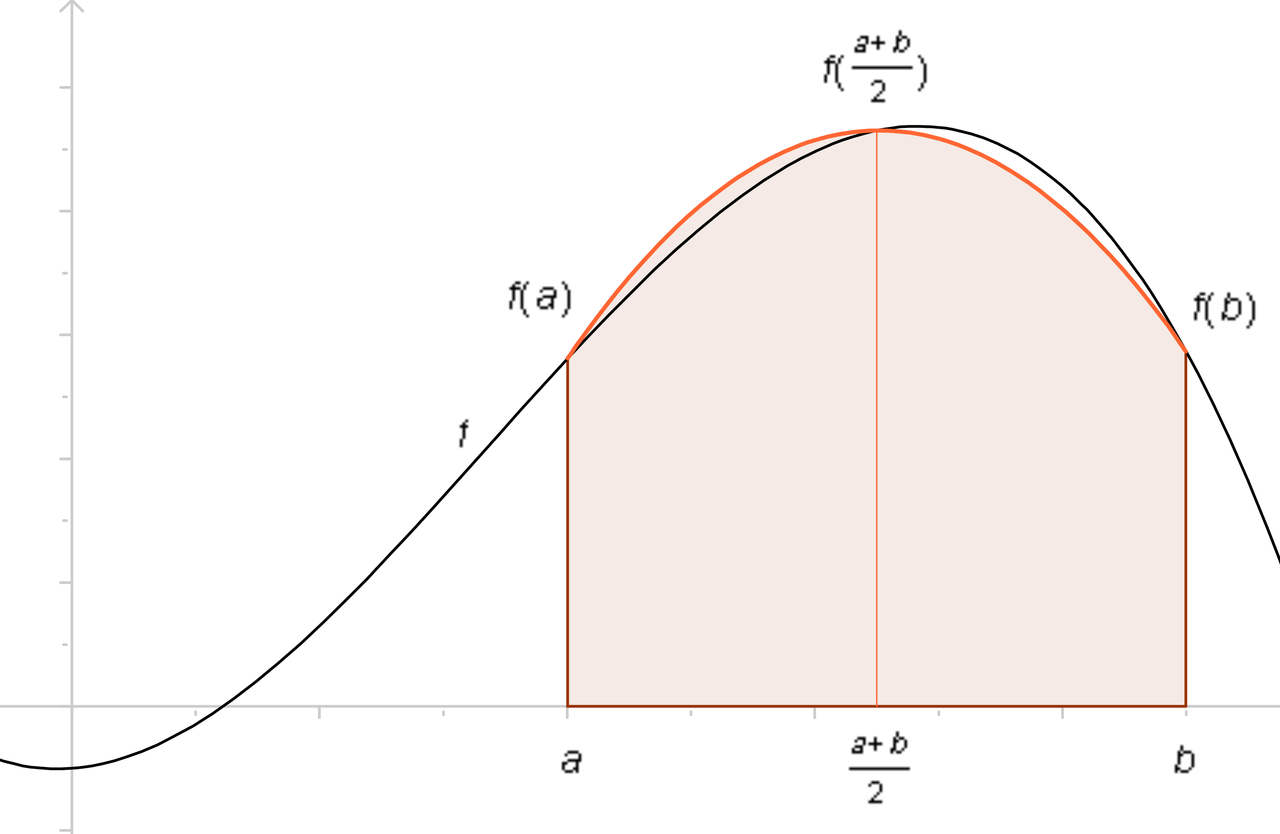
\includegraphics[width=0.5\textwidth]{figure_man/newton_cotes_2.png}
\begin{footnotesize}
\url{https://de.wikipedia.org/wiki/Simpsonregel}\\
Approximation of the integral of $f$ in $[a, b]$ using a polynomial of degree $m = 2$. Three grid points are needed.
\end{footnotesize}
\end{center}

\end{vbframe}

\begin{vbframe}{Polynomial Interpolation}

\begin{itemize}
\item \textbf{Find}: Polynomial interpolation $p_m(x) = \sum_{i = 0}^m a_i x^i$ of degree $m$
\item \textbf{Required}: Evaluation at $m + 1$ data points $(x_{0} = a, x_1, ..., \ldots, x_{m} = b)$
\item At these data points the function values of the polynomial and the function $f$ must be identical, i.e. $p_m(x_k) = f(x_k)$ for $k = 0, 1, ..., m$ or equivalently using the \textbf{Vandermonde} matrix
\begin{footnotesize}
$$
\begin{pmatrix}
1 & x_0 & \hdots & x_0^m \\
\vdots & \vdots & \ddots & \vdots \\
1 & x_m & \hdots & x_m^m \\
\end{pmatrix}
\begin{pmatrix}
a_0 \\ \vdots \\ a_m
\end{pmatrix}
=
\begin{pmatrix}
f(x_0) \\ \vdots \\ f(x_m)
\end{pmatrix}
$$
\end{footnotesize}

\item \textbf{Existence and uniqueness}: If the matrix is regular, the system of equations can be solved \textbf{uniquely}. The matrix is regular if the grid points $x_k, k = 1, ..., m$ are pairwise distinct.
\end{itemize}


\framebreak

The polynomial interpolation can be determined by the solution of the equation system above. However, the effort is high (solution of the LES is $\order(n^3)$).

\lz

The polynomial interpolation can also be defined by using \textbf{Lagrange polynomials}:

$$
L_{im}(x) = \prod_{j = 0,\, j \not= i}^m \frac{x - x_{j}}{x_{i} - x_{j}}, \quad i = 0, 1, ..., m
$$

The polynomial interpolation is:

$$
p_m(x) = \sum_{i = 0}^m L_{im}(x)f(x_{i})
$$

\framebreak


\begin{footnotesize}
%\vspace*{0.3cm}
With:
\vspace*{-0.6cm}
$$
L_{im}(x_k) = \prod_{j = 0,\, j \not= i}^m \frac{x_k - x_{j}}{x_{i} - x_{j}} = \begin{cases}
 1 & \text{if } k = i \\
 0 & \text{if } k \neq i
\end{cases}
$$
\end{footnotesize}

\begin{footnotesize}
\textbf{Example:} Let $m = 3$ and we calculate $L_{i3}$ for $i = 2$
\begin{eqnarray*}
L_{23}(x_k) &=& \prod_{j = 0,\, j \not= 2}^3 \frac{x_k - x_{j}}{x_2 - x_{j}} = \frac{x_k - x_0}{x_2 - x_0} \cdot \frac{x_k - x_1}{x_2 - x_1} \cdot \frac{x_k - x_3}{x_2 - x_3}
\end{eqnarray*}

For $k = i = 2$ all factors are $1$

\vspace*{-0.3cm}
\begin{eqnarray*}
L_{23}(x_2) &=& \frac{x_2 - x_0}{x_2 - x_0} \cdot \frac{x_2 - x_1}{x_2 - x_1} \cdot \frac{x_2 - x_3}{x_2 - x_3} = 1 \cdot 1 \cdot 1 = 1
\end{eqnarray*}

and for $k \ne 2$, e.g. $k = 1$, one factor is $0$ and thus the whole product will be $0$

\begin{eqnarray*}
L_{23}(x_1) &=& \frac{x_1 - x_0}{x_2 - x_0} \cdot \underbrace{\frac{x_1 - x_1}{x_2 - x_1}}_{= 0} \cdot \frac{x_1 - x_3}{x_2 - x_3} = 0
\end{eqnarray*}

\end{footnotesize}


%\framebreak
\begin{footnotesize}
So the polynomial is actually the polynomial interpolation through $(x_k, f(x_k))$

\vspace*{-0.3cm}

$$
p_{m}(x_k) = \sum_{i = 0}^m L_{im}(x_k)%_{\begin{footnotesize}\substack{1 \text{ for } ~ k = i\\ 0  \text{ else}}\end{footnotesize}}
f(x_i) = f(x_k) \quad \text{for k = 0, 1, ..., m}
$$
\end{footnotesize}




% \framebreak
%
% Allgemein lautet das Interpolationspolynom $p_m$ vom Grad $m$ zur Funktion $f$ mit Stützstellen $x_0, x_1, ..., x_m$
%
% $$
% p_m(x) = \sum_{i = 0}^m L_{im}(x)f(x_{i}) \quad \text{ mit } \quad
%   L_{im}(x) = \prod_{j = 0,\, j \not= i}^m \frac{x - x_{j}}{x_{i} - x_{j}}.
% $$


\end{vbframe}

\begin{vbframe}{Newton-C\^{o}tes}

Instead of $f$ we now integrate the polynomial $p_m$:
\begin{eqnarray*}
I(p_m) &=& \int_{a}^{b} p_m(x)~dx = \int_{a}^{b} \sum_{i = 0}^m L_{im}(x)f(x_{i})~dx \\
&=& \sum_{i = 0}^m f(x_{i}) \underbrace{\int_{a}^{b}  L_{im}(x)~dx}_{:=w_{im}}
\end{eqnarray*}

So the integral of $p_m$ on $[a, b]$ is defined by

$$
I(p_m) = \sum_{i = 0}^m w_{im} f(x_{i})
$$

with weights $w_{im} = \int_a^b L_{im}(x)~dx$.

\framebreak

Using equidistant grid points, i.e. $x_i = a + i \cdot h, i = 0, 1, ..., m$ with $h = \frac{b - a}{m}$, the formula can be further simplified.

\lz

When calculating the weights, we use integration by substitution $\int_{\varphi(0)}^{\varphi(m)} L_{im}(x) dx = \int_0^m L_{im}(\varphi(x))\cdot \varphi'(x)~dx $ with $\varphi(x) = x \cdot h + a$.

Since $\varphi(0) = a$ and $\varphi(m) = b$, the following holds

\begin{footnotesize}
\begin{eqnarray*}
w_{im} &=& \int_{\varphi(0)}^{\varphi(m)} L_{im}(x)~dx =  \int_0^m L_{im}(x \cdot h + a) \cdot h ~dx = \int_0^m \prod_{j = 0,\, j \not= i}^m \frac{x - j}{i - j} \cdot \frac{b - a}{m}~dx
\end{eqnarray*}
\end{footnotesize}

In the last step the fact that $x_i = i \cdot h + a$ was exploited

\begin{footnotesize}
\begin{eqnarray*}
L_{im}(x \cdot h + a) &=& \prod_{j = 0,\, j \not= i}^m \frac{x \cdot h + a  - x_{j}}{x_{i} - x_{j}} = \prod_{j = 0,\, j \not= i}^m \frac{x \cdot h + a  - (j \cdot h + a)}{i \cdot h + a - (j \cdot h + a)} = \prod_{j = 0,\, j \not= i}^m \frac{x - j}{i - j}
\end{eqnarray*}
\end{footnotesize}

\framebreak

% Die \textbf{Newton-C\^{o}tes}-Formel für die Approximation des Integrals der Funktion $f$ auf $[a, b]$ lautet
%
% $$
% \int_a^b f(x)~dx \approx \int_a^b p_m(x)~dx = (b - a) \sum_{i = 0}^m w_{im} f(x_i),
% $$
%
% wobei
%
% $$
% w_{im} = \frac{1}{b - a} \int_a^b L_{im}(x)~dx
% $$
%
% die Gewichte und $m$ den Polynomgrad bezeichne.
%
% \framebreak

The Newton-C\^{o}tes formula for equidistant grid points is given by

$$
Q_m(f) = \int_a^b p_m(x)~dx = (b - a)\sum_{i = 0}^m w_{im} f(x_i),
$$
with weights
$$
w_{im} = \frac{1}{m} \int_0^m \prod_{j = 0,\, j \not= i}^m \frac{x - j}{i - j} ~ dx,
  \quad \text{ for } \quad 0 \leq i \leq m.
$$

For a given polynomial of degree $m$ the weights have to be calculated (or looked up) only once, and the formula can be generalized to all possible intervals $[a, b]$.

\framebreak

\textbf{Example:} For $m = 1$, two grid points are needed $\to$ $x_0 = a$, $x_1 = b$.

\vspace{0.2cm}

Calculation of the weights for the integral $[0, 1]$:

\vspace*{-0.3cm}

\begin{eqnarray*}
w_{01} &=& \int_0^1 \left( \frac{x - 1}{0 - 1} \right)~dx = \int_0^1 (1 - x)~dx = \frac{1}{2} \\
w_{11} &=& \int_0^1 \left( \frac{x - 0}{1 - 0} \right)~dx = \int_0^1 x~dx = \frac{1}{2} \\[0.3cm]
\end{eqnarray*}

\vspace*{-0.3cm}

So the formula is given by

\vspace*{-0.2cm}

\begin{eqnarray*}
I(f) \approx I(p_1) &=& (b - a)\cdot (w_{01} \cdot f(x_0) +  w_{11} \cdot f(x_1))  \\
&=& (b - a)  \cdot \frac{f(a) + f(b)}{2}
\end{eqnarray*}


\framebreak

The approach is also called \textbf{trapezoidal rule}.

\begin{center}

\includegraphics[width=0.5\textwidth]{figure_man/trapezregel.png}
\begin{footnotesize}
\url{https://de.wikipedia.org/wiki/Trapezregel}\\
Approximation of the integral of $f$ on $[a, b]$ using polynomials of degree $m = 1$ (trapezoidal rule).
\end{footnotesize}
\end{center}

\end{vbframe}


\begin{vbframe}{Open vs. closed Newton-C\^{o}tes}

We distinguish between:

\begin{itemize}
\item \textbf{Closed} Newton-C\^{o}tes formulas: interval margins $a$ and $b$ are used as grid points for the polynomial interpolation. Usually equidistant nodes are used as grid points, $x_i = a + i \cdot h$, $i = 0, ..., m$ with $h = \frac{b - a}{m}$
\item \textbf{Open} Newton-C\^{o}tes formulas: interval margins $a$ and $b$ are \textbf{not} used as grid points for the polynomial interpolation. Usually equidistant nodes $x_i = a + i\cdot h$, $i = 1, ..., m + 1$, $h = \frac{b - a}{m + 2}$ are used.
\end{itemize}

\end{vbframe}

\begin{vbframe}{Weights of the Newton C\^{o}tes}

\begin{center}
\begin{table}
\small
\begin{tabular}{c c| l l l}
m & type & sampling points $^{(*)}$ & $\omega_{im}$ & \\
% FIXME \hline
\\
0 & open & $\frac{1}{2}$ & $1$ & Riemann sum \\
1 & closed & $0, 1$ & $\frac{1}{2}, \frac{1}{2}$ & trapezoidal rule \\
2 & closed & $0, \frac{1}{2}, 1$ & $\frac{1}{6}, \frac{4}{6}, \frac{1}{6}$ & Simpson's rule \\
3 & closed & $0, \frac{1}{3}, \frac{2}{3}, 1$ & $\frac{1}{8}, \frac{3}{8}, \frac{3}{8}, \frac{1}{8}$ & 3/8-rule \\
4 & closed & $0, \frac{1}{4}, \frac{2}{4}, \frac{3}{4}, 1$ & $\frac{7}{90}, \frac{32}{90}, \frac{12}{90}, \frac{32}{90}, \frac{7}{90}$ & Milne rule \\
\vdots & \vdots & \vdots & \vdots &\\
\end{tabular}
\end{table}
\end{center}

\begin{footnotesize}
$^{(*)}$ The grid points are only valid for integration on $[0, 1]$. For general integration limits the grid points are $a + x_i \cdot (b - a)$.
\end{footnotesize}

\end{vbframe}

\begin{vbframe}{Newton-C\^{o}tes: Quadrature error}

The interpolation error can generally be represented by
\vspace*{-0.3cm}
$$
f(x) - p_m(x) = \frac{1}{(m + 1)!} f^{(m + 1)}(\xi) \cdot \prod_{i = 0}^m (x - x_i),
$$

for an intermediate point $\xi \in [a, b]$. With this, the quadrature error can be generally derived by

\vspace*{-0.3cm}
\begin{eqnarray*}
E(f) &=& \int_a^b p_m(x) - f(x) ~dx = - \frac{1}{(m + 1)!} f^{(m + 1)}(\xi) \int_a^b \prod_{i = 0}^m (x - x_i) ~ dx
\end{eqnarray*}

%\framebreak
\vspace*{0.3cm}
\textbf{Example:} Trapezoidal rule

%\lz

\vspace*{-0.3cm}
\begin{eqnarray*}
E(f) &=& \int_a^b p_m(x) - f(x) ~dx = - \int_a^b \frac{1}{2!} f^{(2)}(\xi) (x - a)(x - b) ~dx\\
&=& - \frac{f^{(2)}(\xi)}{2} \int_a^b (x - a)(x - b)~dx = \frac{1}{12} (b - a)^3 \cdot f^{(2)}(\xi)
\end{eqnarray*}

\end{vbframe}

\begin{vbframe}{Composite rule}

Interpolation with a polynomial of higher degree allows for more flexibility. However, the polynomial function \textbf{oscillates} stronger near the interval boundaries (Runge's phenomenon).

\begin{center}
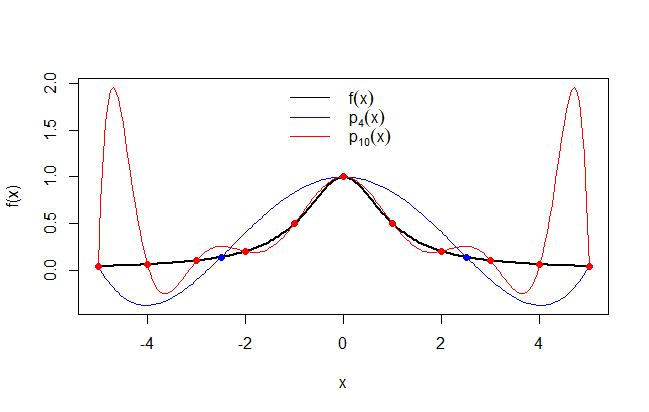
\includegraphics[width = .8\textwidth]{figure_man/Runge.png}
\end{center}


\framebreak

In addition, many Newton-C\^{o}tes formulas have negative weights for degree $\geq 8$, which entails the risk of cancellation.

\lz

Therefore, it is common to divide larger integration intervals $[a, b]$ into $n$ sub-intervals and apply the Newton-C\^{o}tes formula with a lower polynomial degree on each of these sub-intervals. Then, the individual results for the sub-intervals are added up.

\lz

In numerical integration this is known as the \textbf{composite rule}.

\framebreak

\textbf{Degree $m = 1$:} $f$ is approximated in the intervals $[x_i, x_{i + 1}]$ by linear functions (trapezoidal rule)

\begin{center}
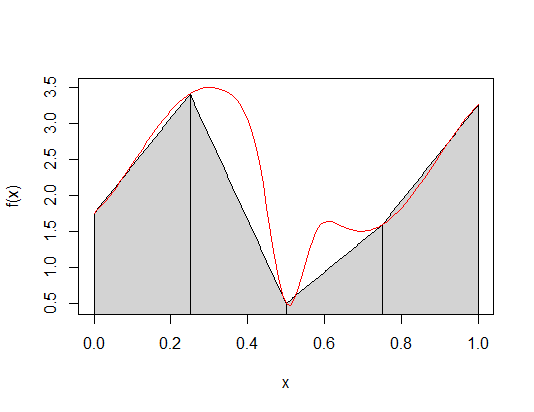
\includegraphics[width = .7\textwidth]{figure_man/deg1.png}
\end{center}

%<<out.width = '90%', fig.align = "center", include = FALSE>>=
%fun = function(x) {
%  -1 * (sin(2 * (4*x - 2)) + 2 * exp(-16^2 * (x - 0.5)^2)) + 2.5
%}
%curve(fun, 0, 1, col = "red", ylab = "f(x)")
%@


%<<out.width = '80%', fig.align = "center", echo=F>>=
%newcot(fun, 0, 1, n = 4, m = 1, plot = TRUE)
%@

\framebreak

\textbf{Degree $m = 2$:} $f$ is approximated in the intervals $[x_i, x_{i + 1}]$ by quadratic functions (Simpson's rule)


\begin{center}
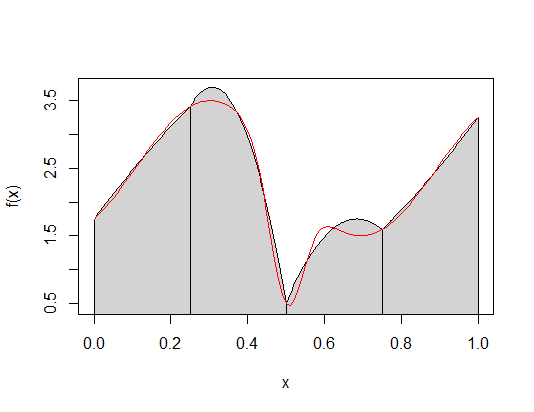
\includegraphics[width = .7\textwidth]{figure_man/deg2.png}
\end{center}

%<<out.width = '80%', fig.align = "center", echo=F>>=
%newcot(fun, 0, 1, n = 4, m = 2, plot = TRUE)
%@

\framebreak

\textbf{Degree $m = 3$:} $f$ is approximated in the intervals $[x_i, x_{i + 1}]$ by polynomials of degree $3$

\begin{center}
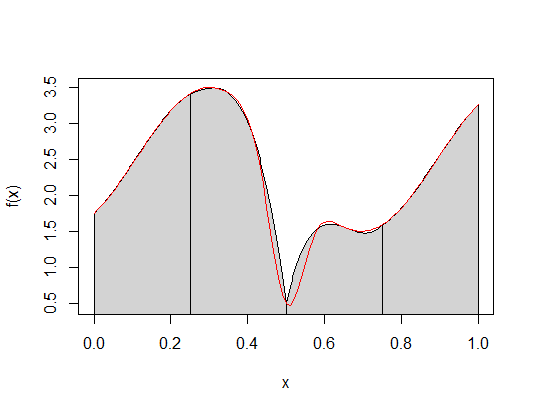
\includegraphics[width = .7\textwidth]{figure_man/deg3.png}
\end{center}

%<<out.width = '80%', fig.align = "center", echo=F>>=
%newcot(fun, 0, 1, n = 4, m = 3, plot = TRUE)
%@

\framebreak

\textbf{Degree $m = 4$:} $f$ is approximated in the intervals $[x_i, x_{i + 1}]$ by polynomials of degree $4$

\begin{center}
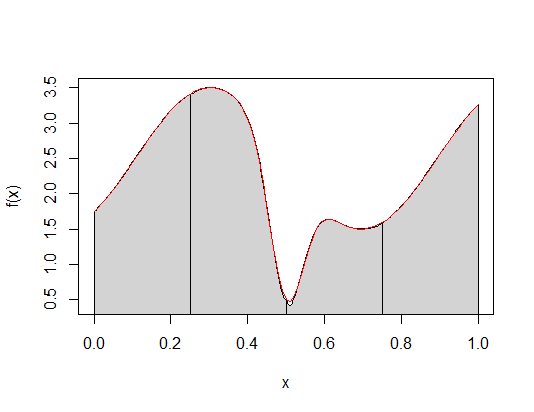
\includegraphics[width = .7\textwidth]{figure_man/deg7.png}
\end{center}

%<<out.width = '80%', fig.align = "center", echo=F>>=
%newcot(fun, 0, 1, n = 4, m = 7, plot = TRUE)
%@

% \framebreak
%
% Für die zusammengesetzten Newton-C\^{o}tes-Formeln gilt die Fehlerabschätzung
%
% $$
% |E(f)| \le \frac{h^{}}
% $$
% |K| \cdot \max_{a \le \xi \le b} |f^{m + 1}(\xi)|

\end{vbframe}



% \framebreak

% <<echo=FALSE>>=
% pinterpol0 = pinterpol

% pinterpol = function(x, y = NULL, degree = 2)
% {
%   if(is.null(y)) {
%     if(is.null(dim(x))) stop("x must be a matrix!")
%     y = x[, 2]
%     x = x[, 1]
%   }
%   f = if(!is.function(y)) {
%     splinefun(x, y)
%   } else y

%   a = min(x, na.rm = TRUE)
%   b = max(x, na.rm = TRUE)

%   xp = seq(a, b, length = degree + 1)




%   w = NULL
%   for(i in seq_along(xp)) {
%     L = 1
%     for(j in seq_along(xp)) {
%       if(j != i) {
%         L = L * (x - xp[j]) / (xp[i] - xp[j])
%       }
%     }
%     w = cbind(w, L)
%   }

%   y = drop(w %*% f(xp))
% }
% @

% <<eval=FALSE>>=
% pinterpol0 = pinterpol

% pinterpol = function(x, y = NULL, degree = 2)
% {
%   if(is.null(y)) {
%     if(is.null(dim(x))) stop("x must be a matrix!")
%     y = x[, 2]
%     x = x[, 1]
%   }
%   f = if(!is.function(y)) {
%     splinefun(x, y)
%   } else y

%   a = min(x, na.rm = TRUE)
%   b = max(x, na.rm = TRUE)

%   xp = seq(a, b, length = degree + 1)
%   #[...]
% @

% \framebreak

% <<eval=FALSE>>=
%   #[...]
%   w = NULL
%   for(i in seq_along(xp)) {
%     L = 1
%     for(j in seq_along(xp)) {
%       if(j != i) {
%         L = L * (x - xp[j]) / (xp[i] - xp[j])
%       }
%     }
%     w = cbind(w, L)
%   }

%   y = drop(w %*% f(xp))
% }
% @

% \framebreak

% <<>>=
% n = 10000
% x = seq(-3, 3, length = 5)
% @

% <<>>=
% system.time(for(i in 1:n) pinterpol0(x, sin))
% system.time(for(i in 1:n) pinterpol(x, sin))
% @


%\end{center}
%


% \end{vbframe}

% \begin{vbframe}{Mittelpunktsregel}

%<<echo=FALSE, include = FALSE>>=
%rectangle = function(f, a, b, n = 20, plot = FALSE, ...) {
%  h = (b - a) / n
%  x = a + (0:(n - 1) + 1/2) * h

%  M = h * sum(f(x))

%  if (plot) {
%    curve(f, a, b, ...)
%    rect(x - h/2, 0, x + h/2, f(x), col = "lightgray")
%    curve(f, a, b, add = TRUE, col = "red", ...)
%    box()
%  } else M
%}
%@


% \vspace*{-0.5cm}
%
% Wir definieren $h:= \frac{b - a}{n}$. Aus der Definition des Riemann-Integrals über Riemann-Summen ergibt sich die Mittelpunktsregel:
%
% $$
% M_n(f) = h\sum\limits_{i=0}^{n-1} f\biggl(\frac{x_{i} + x_{i + 1}}{2}\biggr) = h\sum\limits_{i=0}^{n-1} f(a+(i+ 1/2) h).
% $$


%<<out.width = '70%', fig.align = "center", echo = F, include = FALSE>>=
%rectangle(fun, 0, 1, n = 4, plot = TRUE)
%@

% \framebreak
%
% Das Intervall $[a, b]$ wird so aufgeteilt, dass $(x_0 = a, x_1, ..., x_n = b)$ und $x_{i+1}-x_i=h$. \\
%
% \lz
%
% Als Zwischenstellen dienen die Mittelpunkte $m_i := \frac{x_{i} + x_{i + 1}}{2}$.
%
% \lz
%
% \textbf{Eigenschaften:}
% \begin{itemize}
% \item Für $f \in \continuous^2$: Quadraturfehler $E(f) \le \frac{(b-a)^3 B}{24n^2}$, $B := \sup_{\xi \in [a, b]} f''(\xi)$ \\
%  $\to$ \textbf{Quadratische} Konvergenz
% \item Formel ist exakt für lineares $f$
% \item $n$ Funktionsauswertungen
% \end{itemize}
%
% \framebreak


%<<include = FALSE>>=
%rectangle(fun, 0, 1, n = 10)
%rectangle(fun, 0, 1, n = 100)
%rectangle(fun, 0, 1, n = 1000)
%rectangle(fun, 0, 1, n = 10000)
%@

% \framebreak
%
% \begin{footnotesize}
% \textbf{Herleitung Quadraturfehler} (für $f \in \continuous^2$):\\
%
% Eine Taylorentwicklung von $f$ um $m_i = \frac{x_{i} + x_{i + 1}}{2}$ liefert
%
% $$
% f(x) \approx f(m_i) + f'(m_i)(x - m_i) + \frac{1}{2}f''(\xi_i) (x - m_i)^2.
% $$
%
% mit $\xi_i$ zwischen $m_i$ und $x$. Somit gilt für jeden Summanden von $M_n(f)$
%
% \vspace*{-0.3cm}
%
% \begin{eqnarray*}
% & &\int_{x_i}^{x_{i + 1}} f(x) dx - h \cdot f\biggl(\frac{x_{i} + x_{i + 1}}{2}\biggr) \\
% &\approx& \int_{x_i}^{x_{i + 1}} \biggl[f(m_i) + f'(m_i)(x - m_i) + \frac{1}{2}f''(\xi_i) (x - m_i)^2 \biggr] dx - h \cdot f\biggl(\frac{x_{i} + x_{i + 1}}{2}\biggr) = ... \\
% &=& \underbrace{(x_{i + 1} - x_i)}_{= h} f(m_i) + f'(m_i)\underbrace{\biggl(\frac{1}{2}(x_{i+1}^2 - x_i^2) - m_i(x_{i+1} - x_i)\biggr)}_{= 0} + f''(\xi_i) \frac{1}{3}\biggl(\frac{x_{i+1} - x_i}{2}\biggr)^3 \\
% &-& h \cdot f\biggl(\frac{x_{i} + x_{i + 1}}{2}\biggr) = f''(\xi_i) \frac{1}{3}\biggl(\frac{x_{i+1} + x_i}{2}\biggr)^3 = \frac{1}{24} f''(\xi_i) (\underbrace{x_{i+1} - x_i}_{=h})^3 \le \frac{B}{24} h^3
% \end{eqnarray*}
%
% mit $B := \sup_{\xi_i \in [a, b]} f''(\xi_i)$ (Abschätzung über gesamtes Intervall $[a, b]$).
%
% \framebreak
%
% \end{footnotesize}
%
% Somit gilt die Abschätzung
%
% \begin{eqnarray*}
% E(f) = |I(f) - M_n(f)| &\le& \frac{nBh^3}{24}  =  \frac{(b-a)^3 B}{24n^2}
% \end{eqnarray*}
%
% und es folgt quadratische Konvergenz:
%
% $$
% |I(f) - M_n(f)| \in \order(n^{-2}).
% $$
%
% Die Exaktheit der Methode für lineares $f$ folgt sofort aus obiger Rechnung mit $f''\equiv 0$.
%
% \end{vbframe}
%
% \begin{vbframe}{Trapezregel}

%<<echo=FALSE, include = FALSE>>=
%trapez = function(f, a, b, n = 20, plot = FALSE, ...) {
%  h = (b - a) / n
%  x = a + 0:(n - 1) * h

%  T = h / 2 * sum((f(x) + f(x + h)))

%  if(plot) {
%    curve(f, a, b, ...)
%    for(i in seq_along(x)) {
%      p = cbind("x" = c(x[i], x[i] + h, x[i] + h, x[i]),
%        "y" = c(0, 0, f(x[i] + h), f(x[i])))
%      polygon(p, col = "lightgray")
%    }
%    curve(f, a, b, add = TRUE, col = "red", ...)
%    box()
%  } else T
%}
%@

% \textbf{Idee:} Mittelwert der beiden Riemann - Summen
%
% \begin{eqnarray*}
% T_f(f) &=& \frac{R_n^-(f) + R_n^+(f)}{2} = \sum_{i = 0}^{n - 1} \frac{hf(a + ih) + hf(a + (i + 1)h)}{2}
% \end{eqnarray*}

%<<out.width = '70%', fig.align = "center", echo = FALSE, include = FALSE>>=
%trapez(fun, 0, 1, n = 4, plot = TRUE)
%@

% \framebreak
%
% \textbf{Eigenschaften:}
% \begin{itemize}
% \item Für $f \in \continuous^2$: Quadraturfehler $E(f) \le \frac{(b-a)^3 B}{12n^2}$, $B := \sup_{\xi \in [a, b]} f''(\xi)$ \\
% $\to$ \textbf{Quadratische} Konvergenz
% \item Formel ist exakt für lineares $f$
% \item $n + 1$ Funktionsauswertungen
% \end{itemize}
%
% \lz
%
% Quadraturfehler und quadratische Konvergenz lassen sich für $f \in \continuous^2$ - ähnlich zum Vorgehen bei der Mittelpunktsregel - über eine Taylorentwicklung zeigen.

%<<include = FALSE>>=
%trapez(fun, 0, 1, n = 10)
%trapez(fun, 0, 1, n = 100)
%trapez(fun, 0, 1, n = 1000)
%trapez(fun, 0, 1, n = 10000)
%@

% \begin{eqnarray*}
% T_f(f) &=& \sum_{i = 0}^{n - 1} \frac{hf(a + ih) + hf(a + (i + 1)h)}{2} \\
%   &=& \frac{h}{2}\sum_{i = 0}^{n - 1} [f(a + ih) + f(a + (i + 1)h)] \\
%   &=& \frac{h}{2} [({\color{blue}{f_0}} + f_1) + (f_1 + f_2) + \ldots + (f_{n - 2} + f_{n - 1}) +
%       (f_{n - 1} + {\color{blue}{f_n}})] \\
%   &=& \frac{h}{2} \left[ {\color{blue}{f(a)}} +
%       2 \sum\limits_{i = 1}^{n - 1} f(a + ih) + {\color{blue}{f(b)}} \right].
% \end{eqnarray*}

% \framebreak
%
% Andere Interpretation: Lineare Interpolation von $f$ über jedes Intervall $\quad \Rightarrow \quad$ Fläche von
% Trapez $\frac h2 [f(a + ih) + f(a + (i + 1)h)]$.
%
% \lz
%
% Falls $f$ zwei mal stetig differenzierbar,
% $$
% I(f) - T_n(f) = -(b - a)^3 f''(\xi)/(12 n^2) = -nh^3 f''(\xi) / 12,
%   \,\, \text{ für } \, \xi \in [a, b].
% $$
%
% \lz
% \framebreak

% \end{vbframe}

% \begin{vbframe}{Simpsonregel}

% Quadratische Approximation des Integrals in $[-1, 1]$. Das Integral der quadratischen Approximation kann exakt bestimmt werden.
% \begin{center}
% <<echo=FALSE, fig.height=3.5, fig.width=5, crop = TRUE>>=
% f = function(x) {  dnorm(x + 1, sd = 0.5) * -1 + 1 }
% x = seq(-1, 1, length = 200)
% y = pinterpol(x, f)
% plot(f(x) ~ x, type = "l", ylim = range(f(x), y))
% lines(y ~ x, col = "blue")
% points(c(-1, 0, 1), f(c(-1, 0, 1)), pch = 16)
% legend("bottomright", expression(f(x), Ax^2 + Bx + C), lwd = 1, col = c("black", "blue"),
%   box.col = NA, bg = NA)
% @
% \end{center}




%<<include=FALSE>>=
%simpson = function(f, a, b, n = 10, plot = FALSE, ...) {
%  h = (b - a) / n
%  S = h/6 * (f(a) + f(b) +
%      2 * sum(f(a + (1:(n-1)) * h)) +
%      4 * sum(f(a + (1:n) * h - h/2)))

%  if (plot) {
%    curve(f, a, b, col = "red", ...)
%    for(i in 0:(n - 1)) {
%      x = seq(a + i*h, a + i*h + h, length = 100)
%      y = pinterpol(x, f)
%      p = cbind(c(x, rev(x)), c(y, rep(0, length(x))))
%      polygon(p, col = "lightgray")
%    }
%    curve(f, a, b, col = "red", ..., add = TRUE)
%  } else S
%}
%# simpsonVariante2 = function(f, a, b, n = 20, plot = FALSE, ...) {
%#   if (!(n %% 2 == 0))
%#     n = n + 1
%#
%#   h = (b - a) / n
%#   S = h/3 * (f(a) + f(b) + 4 * sum(f(a + (2*1:(n/2) - 1) * h)) +
%#     2 * sum(f(a + 2*1:((n - 2)/2) * h)))
%#
%#   if (plot) {
%#     plot(c(), xlim = c(a,b), ylim = c(0, 10))
%#     for(i in 0:(n/2 - 1)) {
%#       x = seq(a + i*2*h, a + i*2*h + 2*h, length = 100)
%#       y = pinterpol(x, f)
%#       p = cbind(c(x, rev(x)), c(y, rep(0, length(x))))
%#       polygon(p, col = "lightgray")
%#       abline(v = a + (2*i+1)*h, lty = "dotted")
%#     }
%#     curve(f, a, b, col = "red", ..., add = TRUE)
%#   }
%#   return(S)
%# }
%@

% \textbf{Idee:} Abschnittsweise quadratische Approximation des Integrals.
%
% $$
% \int_a^b f(x)dx \approx \frac{h}{6} \left[ f(a) + f(b) + 2 \sum_{i = 1}^{n - 1} f(a + ih) + 4\sum_{i = 1}^{n}f\left(a + ih - \frac{h}{2}\right) \right]
% $$

%<<out.width = '70%', fig.align = "center", echo = F, include = FALSE>>=
%simpson(fun, 0, 1, n = 4, plot = TRUE, ylim = c(0, 4))
%@


% \framebreak
%
% \textbf{Herleitung der Formel: }
%
% Die Funktion $f$ wird zunächst auf $[-1, 1]$ ersetzt durch seine quadratische Interpolation $Ax^2 + Bx + C$ an den Endpunkten und dem Mittelpunkt:
%
% {\footnotesize
% \begin{eqnarray*}
% A - B + C &=& f(-1) \\
% C &=& f(0) \\
% A + B + C &=& f(1).
% \end{eqnarray*}
% }
%
% Damit ergibt sich für die Koeffizienten
% {\footnotesize
% \begin{eqnarray*}
% % A - B + f(0) &=& f(-1) \\
% % A + B + f(0) &=& f(1) \\[0.3cm]
% % B &=& f(1) - f(0) - A \\[0.3cm]
% % A - (f(1) - f(0) - A) + f(0) &=& f(-1) \\
% % 2A &=& f(-1) + f(1) - 2f(0) \\
% C &=& f(0) \\
% A &=& \frac{f(-1) + f(1)}{2} - f(0) \\
% B &=& \frac{f(1) - f(-1)}{2}.
% \end{eqnarray*}
% }
%
% Als Approximation des Integrals in $[-1, 1]$ ergibt sich somit
%
% {\footnotesize
% \begin{eqnarray*}
% \int_{-1}^{+1} f(x)dx &\approx& \int_{-1}^{+1} (Ax^2 + Bx + C)dx \\
%   &=& \left[ \frac{Ax^3}{3} + \frac{Bx^2}{2} + Cx \right]_{-1}^{+1} \\
%   &=&  \frac{A}{3} + \frac{B}{2} + C - \left( -\frac{A}{3} + \frac{B}{2} - C \right)
%     = \frac{2A}{3} + 2C \\
%     &=& \frac{1}{3}f(-1) + \frac{4}{3}f(0) + \frac{1}{3}f(1)
% \end{eqnarray*}
% }

% \framebreak
%
% Die Approximation des Integrals ist dann
% $$
% \int_{-1}^{+1} f(x)dx \approx \frac{f(-1) + f(1) - 2f(0)}{3} + 2f(0) =
%   \frac{1}{3}f(-1) + \frac{4}{3}f(0) + \frac{1}{3}f(1).
% $$

% \framebreak
%
% Mapping von $[-1, 1]$ nach $[a, b]$ liefert
%
% \begin{eqnarray*}
% u &=& \frac{b - a}{2}x + \frac{b + a}{2} \\
% du &=& \frac{b - a}{2}dx \\
% \frac{2}{b - a} \int_{-1}^{+1} f(x) \frac{b - a}{2}dx &=& \int_{-1}^{+1} f(x)dx \\
% \frac{2}{b - a} \int_{a}^{b} f(u) du &\approx& \frac{1}{3}f(x = -1) + \frac{4}{3}f(x = 0) +
%   \frac{1}{3}f(x = 1) \\
%   &=& \frac{1}{3}f(a) + \frac{4}{3}f\left( \frac{a + b}{2} \right) + \frac{1}{3}f(b).
% \end{eqnarray*}
% $$
% \boxed{\int_{a}^{b} f(x) dx = \frac{b - a}{6} \left[ f(a) + 4f\left( \frac{a + b}{2} \right) + f(b) \right]}
% $$
%
% \framebreak
%
% Zusammengesetzt für $n$ Intervalle:
%
% {\footnotesize
% \begin{eqnarray*}
% \int_a^b f(x)dx &=& \sum_{i = 1}^{n} \int_{a + (i - 1)h}^{a + ih} f(x)dx \\
%   &\approx& \sum_{i = 1}^{n} \frac{h}{6} [f(a + (i - 1)h)
%     + 4f\left(a + ih - \frac{h}{2}\right) + f(a + ih)] \\
%   &=& \frac{h}{6} \left[ f(a) + \sum_{i = 1}^{n - 1} f(a + ih) \,\, + \right. \\
%   && \left. \qquad 4\sum_{i = 1}^{n}f\left(a + ih - \frac{h}{2}\right) + \sum_{i = 1}^{n - 1} f(a + ih) + f(b) \right]
% \end{eqnarray*}
% $$
% \boxed{\int_a^b f(x)dx \approx \frac{h}{6} \left[ f(a) + f(b)
%   + 2 \sum_{i = 1}^{n - 1} f(a + ih)
%   + 4\sum_{i = 1}^{n}f\left(a + ih - \frac{h}{2}\right) \right]}
% $$
% }
%
% \framebreak

% \begin{itemize}
% \item Es findet ein Mapping von $[-1,1]$ in allgemeine Intervalle $[a,b]$ statt.
% \item Um das Integral noch besser annähern zu können, unterteilt man das Intervall $[a,b]$ in Teilintervalle und wendet die Simpsonregel auf die Teilintervalle an.
% \end{itemize}
%
% \textbf{Eigenschaften:}
% \begin{itemize}
% \item Für $f \in \continuous^4$: Quadraturfehler $E(f) \le \frac{(b-a)^5 B}{90n^4}$, $B := \sup_{\xi \in [a, b]} f''(\xi)$ \\
% $\to$ Konvergenzrate der \textbf{Ordnung 4}
% \item Formel ist exakt für kubisches $f$
% \item Zwei Auswertungen pro Intervall nötig \\
% $\to$ Insgesamt $2n + 1$ Funktionsauswertungen
% \end{itemize}
%
% \framebreak

%<<include = FALSE>>=
%simpson(fun, 0, 1, n = 10)
%simpson(fun, 0, 1, n = 100)
%simpson(fun, 0, 1, n = 1000)
%simpson(fun, 0, 1, n = 10000)
%@

% \end{vbframe}

% FIXME Implementierung Newton Cotes nicht in Folien aufgenommen, noch machen?!
%<<include=FALSE>>=
%newcot = function(f, a, b, n = 10, m = 3, open = FALSE, plot = FALSE, ...) {
%  if(m > 10) stop("m > 10 is not allowed!")
%  w = switch(m,
%    "1" = c(1, 1) / 2,
%    "2" = c(1, 4, 1) / 6,
%    "3" = c(1, 3, 3, 1) / 8,
%    "4" = c(7, 32, 12, 32, 7) / 90,
%    "5" = c(19, 75, 50, 50, 75, 19) / 288,
%    "6" = c(41, 216, 27, 272, 27, 216, 41) / 840,
%    "7" = c(751, 3577, 1323, 2989, 2989, 1323,
%      3577, 751) / 17280,
%    "8" = c(989, 5888, -928, 10496, -4540, 10496,
%      -928, 5888, 989) / 28350,
%    "9" = c(2857, 15741, 1080, 19344, 5778, 5778,
%      19344, 1080, 15741, 2857) / 89600,
%    "10" = c(16067, 106300, -48525, 272400, -260550,
%      427368, -260550, 272400, -48525, 106300, 16067) / 598752
%  )
%
%  xp = seq(a, b, length = n + 1)

%  foo = function(w) {
%    n = length(w) + open

%    function(f, a, b) {
%      pos = function(i) a + i * (b - a) / n
%      xp = pos(seq.int(0, length(w) - 1))
%      (b - a) / sum(w) * sum(f(xp) * w)
%    }
%  }

%  bar = foo(w)

%  area = 0
%  for(i in seq_len(n)) {
%    area = area + bar(f, xp[i], xp[i + 1])
%  }

%  if(plot) {
%    y = NULL
%    for(i in seq_len(n)) {
%      x = seq(xp[i], xp[i + 1], length = 100)
%      y = cbind(y, pinterpol(x, f, degree = m))
%    }
%    curve(f, a, b,
%      ylim = range(f(seq(a, b, length = 100)), y), ...)

%    for(i in seq_len(n)) {
%      x = seq(xp[i], xp[i + 1], length = 100)
%      p = cbind(c(x, rev(x)), c(y[, i], rep(0, length(x))))
%      polygon(p, col = "lightgray")
%    }
%    curve(f, a, b, add = TRUE, col = "red", ...)
%    box()
%  }

%  area
%}
%@


% \begin{vbframe}{Adaptive Strategie (Grundidee)}
% \begin{itemize}
% \item Anzahl der Teilintervalle $n$ nicht vom Benutzer gewählt, sondern adaptiv durch Algorithmus.
%
% % \item Knoten nicht äquidistant, sondern rekursiv neue Knoten in Regionen, wo Fehler
% % groß $\quad \Rightarrow \quad$ Brauchen Fehlerabschätzung!
%
% \item $Q_1$ und $Q_2$ seien zwei Quadraturen. $Q_1$ sei die Quadratur auf dem gesamten Intervall,
% $Q_2$ die Summe von 2 Quadraturen auf der linken und rechten Hälfte.
%
% \item Schätzung für Fehler:
% $$
% |Q_1(f) - I(f)| \approx |Q_1(f) - Q_2(f)|
% $$
%
% \item Wenn dies größer als eine vorgegebene Toleranz ist, calle rekursiv auf dem
%   linken und rechten Streifen und gebe die Summe zurück.
%
% \end{itemize}
%
% \end{vbframe}


% \section{Gauß-Quadratur}


% \begin{vbframe}{Gauß-Quadratur}
% Bisher: Mit vorgegebenen Stützstellen $x_i$ berechne die Gewichte $\omega_i$, so dass
% $$
% I(f) \approx Q(f) = \sumin \omega_i f(x_i).
% $$

% \lz

% Grundidee: Wähle $\omega_i$ und $x_i$ so, dass die resultierende Quadraturformel maximale
% Genauigkeit besitzt, i.e., Einschränkung von äquidistant vorgegebenen Stützstellen aufgeben
% und durch freie Wahl von $2n$ $x_i$ und $\omega_i$ Polynome möglichst hohen Grades exakt zu
% integrieren.

% \lz

% Wir betrachten wieder ohne Einschränkungen der Allgemeinheit Integrale im Intervall $[-1, 1]$
% $$
% I = \int_{-1}^1 f(x)dx.
% $$

% \framebreak

% \begin{center}
% <<echo=FALSE>>=
% f = function(x) -1 * x^2 + 1
% curve(f, -1, 0.7, axes = FALSE, ylab = "")
% lines(c(-0.8, -0.8), c(0, f(-0.8)), lty = 2)
% lines(c(0.5, 0.5), c(0, f(0.5)), lty = 2)
% lines(c(-0.8, 0.5), c(f(-0.8), f(0.5)), lty = 2)
% points(c(-0.8, 0.5), c(f(-0.8), f(0.5)), pch = 16)
% lines(c(-0.6, 0.3), c(f(-0.6), f(0.3)), lty = 2, col = "blue")
% lines(c(-0.8, 0.5), c(0.58, 0.97), lty = 2, col = "blue")
% points(c(-0.6, 0.3), c(f(-0.6), f(0.3)), pch = 16, col = "blue")
% lines(c(-0.8, -0.8), c(0, 0.58), lty = 2, col = "blue")
% lines(c(0.5, 0.5), c(0, 0.97), lty = 2, col = "blue")
% lines(c(-0.6, -0.6), c(0, f(-0.6)), lty = 2, col = "blue")
% lines(c(0.3, 0.3), c(0, f(0.3)), lty = 2, col = "blue")
% axis(1, at = c(-0.8, -0.15, 0.5), labels = c(-1, 0, 1))
% box()
% mtext("f(x)", side = 2, line = 1)
% @
% \end{center}

% \framebreak

% \begin{center}
% <<fig.height=3.5, fig.width=5.95>>=
% a = 5
% b = 10
% f = function(x) dnorm(x, mean = 5, sd = 2)
% curve(f, -5, 15)
% @
% \end{center}

% \framebreak

% \begin{center}
% <<>>=
% fn = function(x) {
%   (b - a) / 2 * f((b - a) / 2 * x + (a + b) / 2)
% }
% @

% \lz

% <<crop=TRUE>>=
% par(mfrow = c(1, 2))
% curve(f, a, b)
% curve(fn, -1, 1)
% @
% \end{center}

% \framebreak

% <<>>=
% integrate(f, a, b)
% integrate(fn, -1, 1)
% @

% Also:
% $$
% f(x) := \frac{b - a}{2} g\left( \frac{b - a}{2} x + \frac{a + b}{2} \right),
% $$
% zur Berechnung von
% $$
% I = \int_a^b g(x)dx.
% $$

% \framebreak

% Eine Quadraturformel kann beurteilt werden nach dem Grad der Polynome, die sie
% exakt integriert.

% \lz

% Trapezmethode, $[-1, 1]$:
% $$
% f(x) = \alpha_0x + \alpha_1.
% $$
% $$
% T = Q = \frac{1 - (-1)}{2}(f(-1) + f(1)) = f(-1) + f(1) = 2\alpha_1.
% $$
% \vspace{-3ex}

% \begin{eqnarray*}
% \int_{-1}^{+1} f(x)dx &=& \left[ \frac{\alpha_0}{2}x^2 + \alpha_1x \right]_{-1}^{+1} \\
%   &=& \frac{\alpha_0}{2} + \alpha_1 - \frac{\alpha_0}{2} + \alpha_1 = 2\alpha_1.
% \end{eqnarray*}
% Nachdem $T = 2\alpha_1$ folgt, dass die Trapezmethode mindestens Polynome 1.\ Grades exakt
% integriert.

% \framebreak

% Simpson-Methode, $[-1, 1]$:
% $$
% f(x) = \alpha_0x^3 + \alpha_1x^2 + \alpha_2x + \alpha_3.
% $$
% $$
% S = Q = \frac{1}{3}[f(-1) + 4f(0) + f(1)] = \frac{2}{3}\alpha_1 + 2\alpha_3.
% $$

% \begin{eqnarray*}
% \int_{-1}^{+1} f(x)dx &=& \left[ \frac{\alpha_0}{4}x^4 + \frac{\alpha_1}{3}x^3 + \frac{\alpha_2}{2}x^2 + \alpha_3x \right]_{-1}^{+1} \\
%   &=& \frac{\alpha_0}{4} + \frac{\alpha_1}{3} + \frac{\alpha_2}{2} + \alpha_3 -
%     \frac{\alpha_0}{4} + \frac{\alpha_1}{3} - \frac{\alpha_2}{2} + \alpha_3 \\
%   &=& \frac{2}{3}\alpha_1 + 2\alpha_3.
% \end{eqnarray*}
% Da $S = \frac{2}{3}\alpha_1 + 2\alpha_3$ folgt, dass die Simpson-Methode mindestens Polynome 3. Grades
% exakt integriert.

% \framebreak

% Es gilt:
% \begin{itemize}
% \item Der Genauigkeitsgrad einer Quadraturformel ist höchstens $(2n - 1)$.
% \item Es existiert genau eine Quadraturformel mit $x_i \in [-1, 1]$ welche den maximalen
%   Genauigkeitsgrad besitzt.
% \item Gaußsche Quadraturformeln mit $(n + 1)$ Knoten integrieren Polynome vom Grad
%   $(2n + 1)$ exakt.
% \end{itemize}

% \framebreak

% \textbf{Beispiel:} $n = 2$
% $$
% \int_{-1}^{+1} f(x)dx \approx \omega_1f(x_1) + \omega_2f(x_2)
% $$
% und $f(x)$ ist ein Polynom vom Grad $2 \cdot 2 - 1 = 3$ oder weniger.

% {\small
% \begin{eqnarray}
% \omega_1 \cdot 1 + \omega_2 \cdot 1 &=& \int_{-1}^{+1} 1dx = [x]_{-1}^{+1} = 2 \\
% \omega_1 \cdot x_1 + \omega_2 \cdot x_2 &=& \int_{-1}^{+1} xdx =
% \left[ \frac{1}{2}x^2 \right]_{-1}^{+1} = 0 \\
% \omega_1 \cdot x_1^2 + \omega_2 \cdot x_2^2 &=& \int_{-1}^{+1} x^2dx =
% \left[ \frac{1}{3}x^3 \right]_{-1}^{+1} = \frac{2}{3} \\
% \omega_1 \cdot x_1^3 + \omega_2 \cdot x_2^3 &=& \int_{-1}^{+1} x^3dx =
% \left[ \frac{1}{4}x^4 \right]_{-1}^{+1} = 0
% \end{eqnarray}
% }

% \framebreak

% \begin{itemize}
% \item Aus (2) und (4) erhält man $x_1^2 = x_2^2$ und wegen
% $x_1 \not= x_2 \Rightarrow x_1 = - x_2$.
% \item Damit wird aus (2) $\omega_1 = \omega_2$.
% \item Wegen (1) ist somit $\omega_1 = \omega_2 = 1$.
% \item Aus (3) bekommt man $2x_1^2 = 2/3 \Rightarrow x_1 = 1 / \sqrt{3}$.
% \end{itemize}
% $$
% \int_{-1}^{+1} f(x)dx \approx 1 \cdot f\left( -\frac{1}{\sqrt{3}} \right) +
%   1 \cdot f\left( \frac{1}{\sqrt{3}} \right).
% $$

% \framebreak

% \textbf{Beispiel:}
% $$
% \int_{-1}^{+1} e^x dx = e^{+1} - e^{-1} = 2.350402.
% $$
% Die Trapezregel liefert:
% $$
% \int_{-1}^{+1} e^x dx \approx \frac{h}{2} (f(-1) + f(1)) = e^{-1} + e^{+1} = 3.086161.
% $$
% Mit Integrationsformel für $n = 2$ ergibt sich
% $$
% \int_{-1}^{+1} e^x dx \approx 1 \cdot f\left( -\frac{1}{\sqrt{3}} \right) +
%   1 \cdot f\left( \frac{1}{\sqrt{3}} \right) = e^{-1/\sqrt{3}} + e^{1/\sqrt{3}} = 2.342696.
% $$

% \framebreak

% \begin{itemize}
% \item Im Prinzip könnte man auch die Stützstellen und Gewichte für $n > 2$ bestimmen, allerdings
%   erhält man für die Stützstellen $x_i$ wieder ein nichtlineares Gleichungssystem, dessen
%   Lösung schwierig ist.
% \item Stützstellen sind die Nullstellen von Orthogonalpolynomen.
% \item Legendre, Tschebyscheff, Jacobi, Laguerre, Hermite
%   $$
%   \int_a^b f(x)w(x)dx \approx \sumin \omega_i f(x_i),
%   $$
%   mit $w(x) \geq 0 \,\, \forall x$, $\,\, \int_a^b x^k w(x)dx < \infty \,\, \forall k \geq 0$.
% \item Gauß-Legendre Quadratur $w(x) = 1$
%   $$
%   \omega_i = \int_{-1}^{+1} \prod_{j = 0,\, j \not= i}^m \frac{x - x_j}{x_i - x_j}.
%   $$
% \end{itemize}

% <<message=FALSE, warning=FALSE>>=
% library("statmod")
% gauss.quad(2, kind = "legendre")$nodes
% gauss.quad(2, kind = "hermite")$nodes
% @

% <<>>=
% gauss.quad(5, kind = "legendre")$nodes
% gauss.quad(5, kind = "hermite")$nodes
% @

% \framebreak

% \begin{center}
% \setkeys{Gin}{width=1\textwidth}
% <<echo=FALSE, fig.width=8, fig.height=4.5>>=
% show.roots = function(xlim, jmax = 20, type = "Hermite", ...) {
%   plot(NA, xlim = xlim, ylim = c(0, jmax),
%     ylab = "order", main = type)
%   points(0, 1)
%   for(order in 2:jmax) {
%     quad = gauss.quad(order, tolower(type))
%     points(quad$nodes, rep(order, order))
%   }
% }

% par(mfrow = c(1, 2), mar = c(4.1, 4.1, 4.1, 1.1))
% show.roots(xlim = c(-1,1), type = "Legendre")
% show.roots(xlim = c(-6, 6), type = "Hermite")
% @
% \end{center}
% \end{vbframe}


\begin{vbframe}{Conclusion: Numerical Integration}

\begin{itemize}
  \item In practice, adaptive procedures are often used: the number of sub-intervals to which the Newton-C\^{o}tes formulas are applied is adaptively fine-tuned.
\item The composite Simpson's rule no longer really corresponds to the state-of-the-art, but is certainly
  performant.

  \item There are better methods such as Gaussian quadrature or Gauss–Kronrod quadrature formula
    (not further discussed here).

  \item Impressive convergence rates of some procedures (in 1D), if
    $f$ is sufficiently smooth, otherwise possibly problematic.

\item In principle, the procedures discussed so far can also be generalized to \textbf{higher dimensions}.
\item \textbf{But:} Computing effort increases exponentially with dimension $d$ (\textit{curse of dimensionality}).
\end{itemize}


\end{vbframe}


\endlecture
\end{document}
